%%This is a very basic article template.
%%There is just one section and two subsections.
% \documentclass{article}
%\documentclass[phd,ilcc,twoside]{infthesis}
\documentclass[bsc,logo, abbrevs]{infthesis}
\course{Institute for Language, Cognition and Computation}
\project{\textbf{Supervisor}: Prof. XYZ}

% This package is for times font
\usepackage{times}

% Adjust tables
\usepackage{adjustbox}

% This package is for Informatics thesis style
\usepackage{eushield}

% This package is for your references
\usepackage[numbers]{natbib}

% This package is for figures
\usepackage{graphicx}

% This package is for urls
\usepackage{url}

%Prevents placing floats before a section.
\usepackage[section]{placeins}

% Degree command
\usepackage{gensymb}

% For symbols and equations 
\usepackage{latexsym}
\usepackage{amsmath}
\usepackage{acronym}

% Using urls

\usepackage{url}

% Referencing in center
\usepackage{csquotes}
\renewcommand{\mkbegdispquote}[2]{\itshape}

%% Information about the title, etc.
\title{Personalized Air Quality Visualization and Tracking}
\author{Alberto Vazquez Martinez}

%% Specify the abstract here.
%\abstract{%
%
%Abstract for my Report
%}

\begin{document}

%% First, the preliminary pages
\begin{preliminary}

\maketitle

%% Create the table of contents
\standarddeclaration
\dedication{To my mummy.}
\tableofcontents
\listoffigures
\listoftables
\begin{accron}\begin{acronym}[MPC] % Give the longest label here so that the list is nicely aligned
\acro{MPC}{model predictive control}
\acro{TLA}{Three Letter Acronym}
\acro{COMEAP}{Committee on the Medical Effects of Air Pollutants}
\acro{DEFRA}{Department for Environment Food and Rural Affairs}
\acro{NO2}{Nitrogen Dioxide}
\acro{O}[O\textsubscript{3}]{Ozone}
\acro{SO}[SO\textsubscript{2}]{Sulphur Dioxide}
\acro{NO}[NO\textsubscript{x}]{Nitrogen Oxides}
\acro{PM}{Particle Matter}
\acro{PM}[PM\textsubscript{10}]{Particle Matter 10 micrometer}
\acro{PM}[PM\textsubscript{2.5}]{Particle Matter 2.5 micrometer}
\acro{IaaS}{Infrastructure as a service}
\acro{UI}{User Interface}
\acro{API}{Application Programming Interfaces}
\acro{CMEAP}{Committee on the medical effects of air pollutants}

\end{acronym}\end{accron}

\end{preliminary}

\chapter{Introduction}
Breathing fresh air is a right that everyone should have.
In recent years air quality has taken on an increasingly important role in people's lives as well as government institutions which are increasingly aware of the hazards of air pollution. In Scotland alone there are in total 32 ``pollution zones'' that are considered to breach European safety standards \cite{Foe-scotland.org.uk} \cite{OKScotland2015}. The negative impact of poor air on our health, diminishing our life quality and causing cardiovascular and respiratory diseases is of greater concern. As such, new air quality monitoring sensors are being developed and deployed. Some of them are in fixed locations, whilst others are carried around. Data is becoming more available and fine-grained providing a further capability to enable educated decisions.

Through this new outsourced data, it is possible to tackle the pollution problem by taking a  more personalised approach as ``everyone has different needs and lifestyles that expose them differently to pollution'' \cite{Vazquez2016}. Different population groups are more vulnerable than others. For example, children are more affected than adults because their lungs are still developing. Furthermore, people with respiratory diseases suffer from aggravated symptoms because their airways get irritated with spikes in air pollution. The way data is presented and disseminated to the public is crucial part of the solution. Therefore, digitally enabled visualisation is an excellent tool that unleashes the full potential of data; as new technologies are available to extract, filter, display and animate it evoking the interest and attention of the people while providing unique experiences and mechanisms to improve their lives.

\iffalse
The effects of air pollution on human health are still complex to understand and there is much research ongoing on the combination short and long term effects upon a person's health. 
\fi
\section{Aims and Objectives}
The first aim of this project is to review current approaches to air quality data dissemination and visualisation. Furthermore, this project examines the current needs of pollution-sensitive and non-sensitive users in relation to a new air-quality data dissemination tool to accomplish the main goal: to develop and implement a mobile application to visualise air quality data in a useful and understandable way.

Another important objective is to take on a more user-centred approach whilst achieving this main goal, by bearing in mind the users as co-designers and stakeholders throughout three different design iterations of the product for the creation of a final prototype that reflects more accurately the user needs and thoughts.

\iffalse
DATA -> APP -> USEFUL -> PERSONAL -> DECISION SUPPORT -> DESIGNED BY PEOPLE
\fi
\input{1-introduction/3-Challenges}
\section{Dissertation Outline}
This dissertation is structured as follows: 
 
\bigskip
 Chapter 2: Background
\bigskip

This chapter discusses relevant background topics key to understanding the dissertation. It explains the project's importance in the context of the pollution problem, including definitions to follow the basic air quality dissemination terms and related health issues. Past approaches for visualising are also discussed and critically evaluated, as well as explaining in detail what is meant by data visualisation and how to achieve it from a decision support perspective.
 
\bigskip
 Chapter 3: Methodology
\bigskip
  
This chapter describes the methodology and processes that have been used throughout the project. It describes how the development was addressed not only from a human-computer interaction perspective but as well from a software engineering perspective. 
  
\bigskip  
 Chapter 4: Analysis and Design
\bigskip

The analysis and design of the system are  both addressed in this chapter. A detailed analysis of the current needs of a new air quality application are presented, as well as explaining the design and infrastructure choices made for achieving the project goal in a way all stakeholders are considered. The first application prototype is presented.
 
\bigskip
Chapter 5: Implementation
\bigskip

This chapter describes how the required infrastructure and software components were set-up to proceed with the implementation of the final two prototypes, as well as the transitional choices that resulted from the user-centred development approach.

\bigskip
 Chapter 6: Evaluation
\bigskip

The final technical and user evaluations are presented in this chapter by describing how well the defined requirements in Chapter 4 were met with quantitative and qualitative methods.

\bigskip
 Chapter 7: Conclusion
\bigskip

This chapter looks at the aims of the dissertation from an integrative perspective highlighting what has been accomplished so far and giving recommendations for future research.
\chapter{Background}
\section{Air Quality}
\subsection{Air pollution and its health effects}
Air pollution can be defined as a group of chemicals present in the atmosphere that are harmful to humans, animals or vegetation. It is mainly caused by human activities, such as transport, industry, or agriculture. But it can also be influenced by other natural sources. Understanding air pollution is important because many health consequences result from high pollution levels. 
\begin{figure}[h]
  \centering
  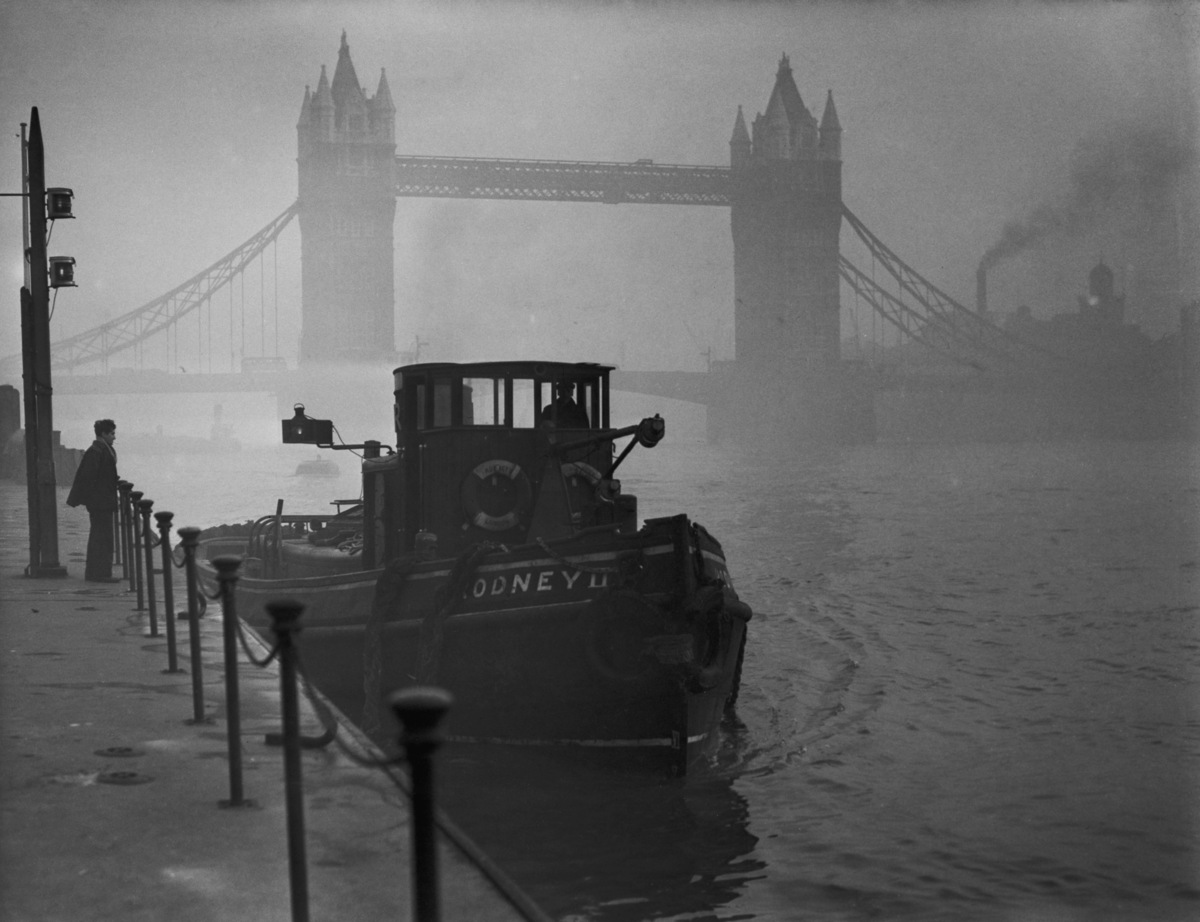
\includegraphics[scale=.8]{images/great_smog.jpg}
  \caption[Great smog of 1952]{Great smog of 1952 \cite{ElliotWagland2013}}
  \label{fig:interaction_design}
\end{figure}

One historic event which caused huge consequences is known as the great smog of 1952. Thousands of people died in Greater London due to exposure over several days to a highly contaminated atmosphere, and many others became ill or experienced retarded symptoms \cite{Bell2008}. The fog originated from coal burning, vehicle exhaust and other atmospheric factors. Although many human activities introducing pollution have changed since then, it became evident the immediate and retarded health impact of pollution. 

Pollution particles can be categorised into gaseous pollutants, persistent organic pollutants, heavy metals and particulate matter. They vary in their chemical composition, emission sources and impact on health. 

Gaseous pollutants are sulphur dioxide (\SOTWO), nitrogen oxides (\NOX), carbon monoxide (CO), ozone (\OTHREE) and volatile organic compounds (VOCs). The principal source of gaseous pollutants is combustion of fossil fuels and diesel emission from vehicles. Nitrogen oxides (\NOX) is a general term that includes nitric oxide (NO) and nitrogen oxide \NOTWO. Gaseous pollutants can affect our health by inflaming the airways and lungs, and in the long term, affect the function of the lungs \cite{AirQualityExpertGroup2004} \cite{WHO2003}.

Particulate matter (PM) is a mixture of solid and liquid particles (such as sulphate, nitrates, ammonia, sodium chloride, black carbon, mineral dust and water). PM are categorised according to their diameter size measured in microns (\SI{}{\micro\metre}, one millionth of a metre). Particles smaller than 10 microns (\PMTEN) are known as coarse particles, smaller particles with a size of up to 2.5 and 1 microns (\PMTWO and \PMONE) are known as fine and ultra-fine particles respectively. They are differentiated in sizes because it dictates their aerodynamic properties, that is, how they are transported into the air, as well as how far they can get into the respiratory system. According to the World Health Organization, PM is the most harmful pollutant because it can pass through the nose and throat and enter the lungs, there is also evidence that it is associated with risk of cardiovascular disease \cite{Polichetti2009}. 

Air quality is also affected by pollution mixture in further complex chemical structures and by temperature and humidity conditions. \NOTWO, PM and O\textsubscript{3}  pollutants get transformed by atmospheric processes making it hard to evaluate their individual impact. As an example, ground level ozone is produced when sunlight interacts with \NOTWO and volatile organic compounds. Furthermore, \NOTWO and other nitrogen oxides also contribute to PM generation, making \NOX a particularly concerning pollutant.

\subsection{Air quality data dissemination}
Openly published air quality data aimed to have informed and aware citizens that could take part into more sustainable and environmental choices. \quotes{Yet, what was lacking (and it still is), is a model for effective communicating of environmental information to the public} \cite{Thinh2007}. Terms like assessment, limit values, target values and concentration, among others, are commonly used by air quality data publishers to describe the current or forecasted quality status; however, there is not general agreement on how air quality information should be disseminated to the general public in a way it is understood immediately and intuitively. 

In general it is complex to categorise and establish measures for the different components of air pollution due their heterogeneous nature and the chemical reactions that occur between them. Measurement methods and units vary from institution to institution and regulation standards can be specific for each country, which may give rise to ambiguity. Furthermore, much of the available data is represented in a tabular format, including various information for individual pollutants, as exemplified in table \ref{tab:pollution_tabular_data}. This table was extracted from the  Department for Environment Food and Rural Affairs (DEFRA) website \cite{DepartmentforEnvironmenta}, and shows measures related to the air quality from a sensing station located in Deaconess Garden in the south of Edinburgh. At first sight it table arises some questions for the novice on air-quality trying to crack the data. Firstly, the pollution codes such as PM2.5, PM10, NO2, NOX as NO2 and their subtle differences should be understood. Secondly, some measurement units are tagged with the monitoring method used to extract the information, like the TEOM FDMS \footnote{Which indicates that the sensing methods were Tapered Element Oscillating Microbalance and Filter Dynamics Measurement System \cite{Quality2005}} tag. And lastly, it is hard to know which measurements are of more interest given a person's particular circumstances. As stated by Brimblecombe and Schuepbach \cite{P.Brimblecombe2008}, \quotes{many people complain that the information is unintelligible, while some have even seen it as an attempt of government to blind the public with science}.  It is clearly difficult to understand the meaning of the terms and values that are used to represent air quality data to the general public. 

\begin{table}[ht]
\centering
\begin{adjustbox}{width=1.2\textwidth,center=\textwidth}
\begin{tabular}{rlrrrrrrr}
  \hline
 Pollutant & Date & Time & Measurement & Unit & Period & Comment  \\ \hline
    Ozone (O3) & 20/07/2016 & 07:00 & 63.06412 & µg/m3 & Hourly & - \\
    Nitric oxide (NO) & 20/07/2016 & 07:00 & 2.61933 & µg/m3 & Hourly & - \\
    Nitrogen dioxide (NO2) & 20/07/2016 & 07:00 & 27.34875 & µg/m3 & Hourly & - \\
    Nitrogen oxides as nitrogen dioxide (NOXasNO2) & 20/07/2016 & 07:00 & 31.36500 & µg/m3 & Hourly & - \\
	Sulphur dioxide (SO2) & 20/07/2016 & 07:00 & 14.63495 & µg/m3 & Hourly & - \\
	Carbon monoxide (CO) & 20/07/2016 & 07:00 & 0.081494 & mg/m3 & Hourly & - \\
	PM10 particulate matter (Hourly measured) (PM10) & 18/07/2016 & 15:00 & 10.900 & µg/m3 (TEOM FDMS) & Hourly & - No current data. \\
	Non-volatile PM10 (Hourly measured) (Non-volatile PM10) & 19/07/2016 & 07:00 & 26.700 & µg/m3 (TEOM FDMS) & Hourly & - No current data. \\
	Volatile PM10 (Hourly measured) (Volatile PM10) & 19/07/2016 & 07:00 & 5.500 & µg/m3 (TEOM FDMS) & Hourly & - No current data. \\
	PM2.5 particulate matter (Hourly measured) (PM2.5) & 18/07/2016 & 15:00 & 4.300 & µg/m3 (TEOM FDMS) & Hourly & - No current data. \\
	Non-volatile PM2.5 (Hourly measured) (Non-volatile PM2.5) & 19/07/2016 & 07:00 & 16.300 & µg/m3 (TEOM FDMS) & Hourly & - No current data. \\
	Volatile PM2.5 (Hourly measured) (Volatile PM2.5) & 19/07/2016 & 07:00 & 5.000 & µg/m3 (TEOM FDMS) & Hourly & - No current data. \\
	Modelled Wind Direction (Dir) & 19/07/2016 & 24:00 & 50.6 & \degree & Hourly & - No current data. \\
	Modelled Wind Speed (Speed) & 19/07/2016 & 24:00 & 6.2 & m/s & Hourly & - No current data. \\
	Modelled Temperature (Temp) & 19/07/2016 & 24:00 & 14.6 & °C & Hourly & - No current data. \\
	PM10 Ambient Temperature (AT10) & 19/07/2016 & 07:00 & 19.4 & °C & Hourly & - No current data. \\
	PM10 Ambient pressure measured (AP10) & 19/07/2016 & 07:00 & 989.0 & mb & Hourly & - No current data. \\
	PM2.5 Ambient Temperature (AT25 ) & 19/07/2016 & 07:00 & 17.5 & °C & Hourly & - No current data. \\
	PM2.5 Ambient Preasure (AP25) & 19/07/2016 & 07:00 & 988.0 & mb & Hourly & - No current data. \\
   \hline
\end{tabular}
\end{adjustbox}
\caption{Air quality tabular data representation. \cite{DepartmentforEnvironment}}
\label{tab:pollution_tabular_data}
\end{table} 

\subsection{The COMEAP air quality index and health advice}
In order to understand the correlation between air quality data and its effects on human health, the Committee on the Medical Effects of Air Pollutants (COMEAP) developed the air quality index based on health evidence. It is used to communicate real-time air quality levels and their short-term health effects for five selected harmful pollutants: particulate matter (\PMTEN and \PMTWO), ozone (\OTHREE), sulphur dioxide (\SOTWO), and nitrogen dioxide (\NOTWO) as shown in Figure \ref{fig:air_quality_index}. The index employs a colour scale and a number index to inform about how high are the concentrations of each specific pollutant. Four bands are employed: Low, Moderate, High and Very High. 

\begin{figure}[H]
\begin{adjustbox}{width=1\textwidth,center=\textwidth}
  \centering
  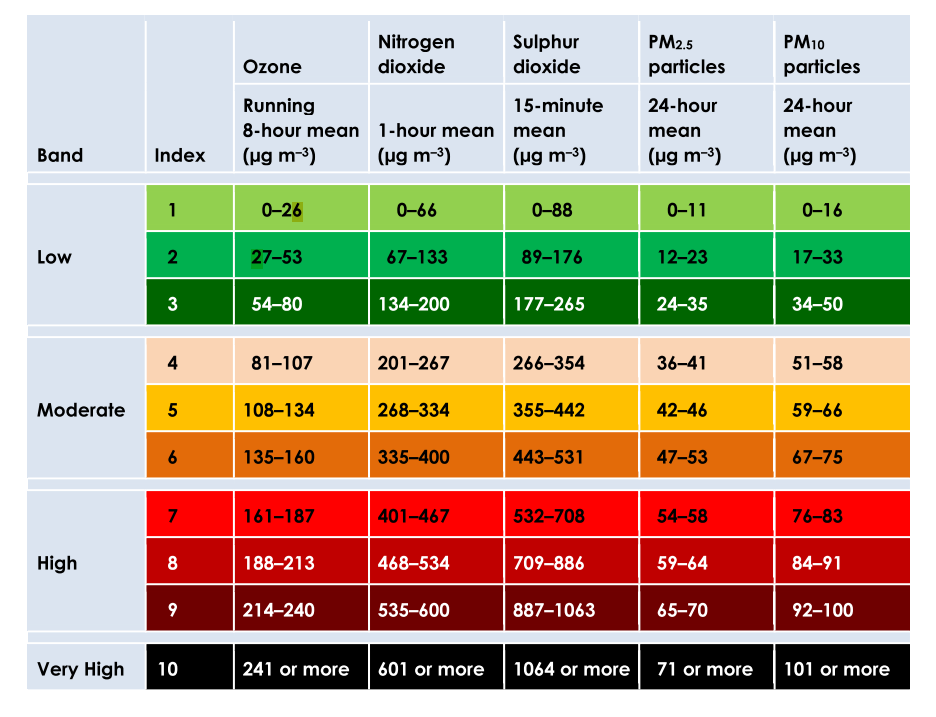
\includegraphics[scale=.8]{images/air_quality_index.png}
\end{adjustbox}
  \caption[The COMEAP air quality index]{The COMEAP air quality index \cite{HealthProtectionAgencyfortheCommitteeontheMedicalEffectsofAirPollutants2011}}
  \label{fig:air_quality_index}
\end{figure}

There is substantial evidence that the elderly, children, and persons that suffer from chronic diseases such as asthma are in greater danger of suffering symptoms and health consequences from lower pollution concentrations than the general public \cite{Koenig1999} \cite{Kampa2008} \cite{Zones2010} . The COMEAP includes such population in their Air Quality Index to give them the opportunity to modify their behaviour and reduce the severity of their symptoms. Furthermore, the air quality index is accompanied by a health advice (Figure \ref{fig:air_quality_health_advice}) which provides specific health messages targeting both population groups, sensitive and non-sensitive providing information about the actions that should be taken to avoid symptoms and health effects.

\begin{figure}[H]
\begin{adjustbox}{width=1\textwidth,center=\textwidth}
  \centering
  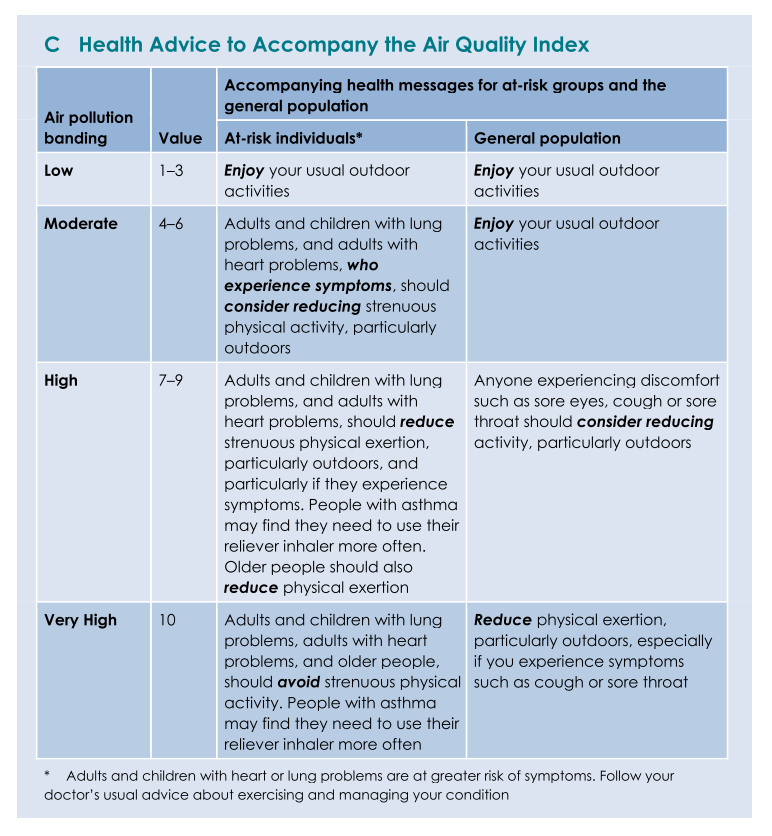
\includegraphics[scale=.8]{images/air_quality_health_advice.png}
\end{adjustbox}
  \caption[Air quality health advice]{Air quality health advice \cite{HealthProtectionAgencyfortheCommitteeontheMedicalEffectsofAirPollutants2011}}
  \label{fig:air_quality_health_advice}
\end{figure}


\subsection{Air quality sensors}

\begin{itemize}

\item Fixed sensors: 

Fixed sensors are installed and maintained by the UK government and local authorities in Scotland. There are of two kinds, automatic sensors from the Automatic Urban and Rural Network (AURN)\footnote{\url{https://uk-air.defra.gov.uk/networks/network-info?view=aurn}}, and non automatic sensors maintained by local Scottish councils. 

	\begin{itemize}
    
    \item Automatic sensors: They produce hourly concentrations and data is sent automatically over the network. They purpose is to check that EU and other regulatory standards are being met as well as informing the public about air quality. These sensors monitor a wide range of pollutants (\NOX, \SOTWO, CO\textsubscript{2}, O\textsubscript{3}, \PMTWO and \PMTEN) which are later collected and processed by Ricardo Energy and Environment \footnote{\url{http://ee.ricardo.com}} and exposed through HTML webpages at the Scottish Air Quality website\footnote{\url{http://www.scottishairquality.co.uk/}} or CSV files provided on demand. 
	\item Non automatic sensors: 
    
    \end{itemize}

\item Portable sensors:

\item Participatory sensors:

Some projects such as CitiSense \cite{Nikzad2012} include users as 'human sensors' by reading their perceptions towards air quality in certain locations. This method aims to get more fine-grained information about air quality and engage the citizens in the pollution problem and its solution. 

\end{itemize}




\section{Air Pollution Health effects}

 The health effects of NO\textsubscript{x} are irritating the lungs and increasing susceptibility to respiratory infections like influenza[].
 According to the World Health Organization, PM is the most harmful pollutant because it can pass through the nose and throat and enter the lungs. PM 
 
Exposure to PM is associated with risk of cardiovascular disease \cite{Polichetti2009}


\section{Decision Support Systems}
\section{Air Quality Applications}
\section{Air Quality Data}
\input{2-background/6-Data-Visualization}
\chapter{Methodology}
In order to accomplish the project aim, it is imperative to select a framework which allows a user inclusive development process as well as a flexible and iterative workflow. The project followed an interaction design model and an agile development methodology. The following sections will give a brief outline of these methods, as well as describe how they have been used throughout the project.
\section{Interaction Design Process}
Interaction design can be briefly defined as "designing interactive products to support people in their everyday working lives" \cite{Sharp2011}. To develop a useful product an understanding of what is needed must be established before and during the development process. This brings new challenges and questions, such as if users understand what are they expecting from a specific product; and, of course, correctly establishing who the users are beforehand. Interaction design process is a strong user-centered methodology, that, correctly carried out will output a product that reflects the real user voice and needs. An user must be understood as the persons that will use the product for the intended goals. The stakeholders are the persons that are involved in the development process influencing the system requirements. For the purposes of this project, the users are the general public who are concerned with air quality and how it can have an impact on their health status. The stakeholders are the secondary agents who have provided an opinion on the capabilities of the system, in this case are my project supervisor and other researchers in the field that can give formative feedback.

As described in Figure \ref{fig:interaction_design}, the interaction design process is carried out with four activities: \begin{itemize}
  \item Identify user needs and establishing requirements
  \item Develop alternative designs
  \item Build interactive versions
  \item Evaluation with users
\end{itemize}

\begin{figure}[h]
  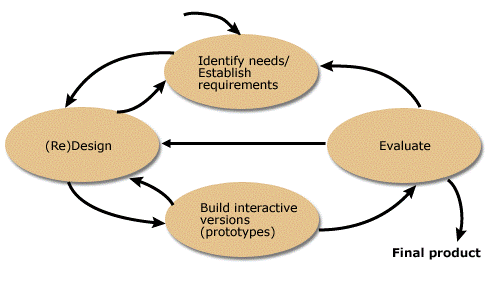
\includegraphics[scale=.8]{images/interatcion-design.png}
  \caption[Interaction design process]{Interaction design process \cite{Sharp2011}}
  \label{fig:interaction_design}
\end{figure}

Identifying needs and establishing requirements is the first and most crucial activity of the process. Its objective is to learn and understand the user needs and communicate them to the developer. According to the chaos report \cite{Group1994}, requirements account for more than the 30\% of the project failure factors, they include lack  of user input, incomplete requirements and specifications, or changes in requirements and specifications. Also its interdisciplinary nature, and contradictions between stakeholders add complexity to this part of the process. To guide it in a more accurate and disciplined manner, it is useful to combine different techniques and methodologies, such as questionnaires, interviews, introspection and brainstorming \cite{Coulin2005}. The selected methods were questionnaires and interviews. Interviews allowed to establish a casual conversation with few potential application users, whereas questionnaires allowed to get different points of views of many potential users of the application. 

A support tool for developing alternative designs is the prototype. It is a physical, or digital outline of a screen or task supported by the product. It allows for different purposes: first, as support for the creative process, allowing the designer to print how is the interface expected to look like and how it will support the intended use cases. Second, as a communication tool for the stakeholders, supporting the flow of ideas between the designer and the people involved in the development. And third, as a testing tool, allowing the designer to get measurable feedback of the capabilities of the product. Prototypes were designed and evaluated in different iterations among the project.
\section{Agile methodology}
The development process followed an agile methodology as a good software engineering practice. The benefit of this approach is that more focus is paid to the product than to the management process. This has proven to be a strong advantage when working on constantly-changing and time-constrained projects such as this dissertation project.
The agile manifesto \cite{Martin2002} establishes four values to guide a development process: 
\begin{displayquote}
\begin{itemize}
  \item Individuals and interactions over processes and tools
  \item Working software over comprehensive documentation
  \item Customer collaboration over contract negotiation
  \item Responding to change over following a plan. 
\end{itemize}
\end{displayquote}

Agility moves the interest in software development towards product functionality rather than product documentation. It recognises that much time can be spent on documenting and planning and stimulates smart resource usage instead by working closely with the stakeholders, responding to change and prioritising software components that have direct interaction with the user. This allows the developer to output iterations to the user for evaluating earlier in the development process.

\iffalse
\subsection{Self-management}
Versioning software was used to manage the workflow of the different components of the system, the repositories are available online in a public GitHub repository. Links
\fi
\section{Evaluation}
Considering that a deliverable of my project dissertation is a mobile application that includes technical and design aspects, the evaluation should be qualitative and quantitative. It should be quantitative to collect measurable indicators of how well the user-requirements were met from a software engineering perspective. Also, qualitative to get an insight from an interaction-design perspective to collect thoughts and reflections about the product.

\subsection{Technical evaluation}
A technical evaluation will ensure that the software behaves as expected during deployment. This will be done by inspecting and debugging the code through the entire development process. Code inspections are performed by visually inspecting the program coded statements and allow for the discovery of logic and coding errors in order to spend less time and effort debugging \cite{Myers2011}. The coding errors that are not discovered on the inspection process will show up when executing the program and may be fixed by debugging. The debugging process finds and corrects suspected errors within the program effortlessly by the use of debugging tools integrated into modern development editors. Once the software development stage has been exhausted, automated tests will be used to discover errors that may still be present.

\subsection{Evaluation with users}
Although designing for usability is the priority, users during the testing phase are expected to use computers and smartphones confidently. Otherwise, tasks within the system will not be carried out independently and may skew gathered results. 

Of particular interest is the level of satisfaction of the app with the user. This will involve collecting measurable indicators of how well the non-functional and functional requirements were met by the application. In other words, to assess how well people can understand and use a product or prototype.

\quotes{This method is accomplished by identifying representative users, representative tasks, and developing a procedure for capturing the problems that users have in trying to apply a particular software product in accomplishing these tasks.} \cite{Scholtz2003} The advantage is the involvement of the user; however, the test attendants should be a representative group of the potential final users of the product. The selected tasks should aim to be as realistic as possible because \quotes{results are based on actually seeing what aspects of the user interface cause problems for representative users}. \cite{Scholtz2003}

\subsection{Design critique}
The objective of including this method is to gather impressions and thoughts about the system and foster an open space to discover what the development of future releases should aim for. According to Blevis et al. \cite{Blevis2007} it allows for understanding the development from the perspective of the user. In this case it will try to understand how the users would include such a development in their daily lives. For instance, if they would be willing to use it on a regular basis because it is attractive and fun to use, or just because they feel it would benefit their health. All of this feedback would give a deeper understanding of the flaws and strengths of the system.

\iffalse
\quotes{Process of discourse on many levels of the nature and effects of an ultimate particular design}. \quotes{Comment on the qualities of an ultimate particular from an holistic perspective, including reason, ethics, and aesthetics as well as minute details of form and external effects on culture}.\cite{Blevis2007}
\fi


\iffalse\section{Out of Scope Issues}\fi
\chapter{Analysis and Design}
The focus of this chapter is to establish and discuss what the software is going to do, and how is going to achieve its intended goals. The actors in defining were from different institutions related to the issues treated by the project. This chapter describes how they were involved as stakeholders, co-designers and evaluators. 

\begin{figure}[h]
\begin{adjustbox}{width=1\textwidth,center=\textwidth}
  \centering
  \includegraphics[scale=1]{images/stakeholders.png}
\end{adjustbox}
  \caption[Colaborators in the project]{Collaborators in the project.}
  \label{fig:stakeholders}
\end{figure}

\section{Users and stakeholders}
As mentioned before, before the start of the development phase, it is important to establish who are the intended users of the application, as well as the stakeholders. 

The following users were depicted for this development:

\begin{itemize}
    \item General public: The general public who is concerned whit the air quality of their environment.
    \item Pollution-sensitive public: People at risk of suffering health consequences due to air pollution.
\end{itemize}

To gain input from different perspectives, the following stakeholders were involved in the development: 

\begin{itemize}
	\item Researchers 
    \begin{itemize}
      \item Asthma UK researchers: Meetings were arranged with various researchers of the Asthma UK group and. They were involved early in the design of a first prototype, by providing ideas and highlighting issues that may arise from a medical researcher perspective. The researchers were:  Dr Aziz Sheikh, director of the research group, Dr Soyiri Ireneous, and Dr Lynn Morrice. They belong as well to the Usher Institute of Population Health Sciences and Informatics\footnote{\url{http://www.ed.ac.uk/usher}}
      
    The following issues were raised in the meetings:
      \begin{itemize}
          \item Based on their experience further considerations should be taken when designing applications that rely on user input.
          \item Review past approaches/work to avoid known problems.
          \item An application should give actionable feedback rather than just displaying information.
          \item Ask the users in order to find out what they want.
      \end{itemize}
      \item University of Edinburgh School of Informatics researchers: My supervisor Dr Ewan Klein and Catherine Magill, both researchers at the University of Edinburgh and part of the Edinburgh living lab which focus is on open data and how it impacts on behaviour and society. They also have a strong background in participatory design. They were asked to provide feedback on inner prototypes.
	\end{itemize}
	\item Domain experts    
   \begin{itemize}
      \item Chief Technology Officer: Simon Chapple acts as CTO of Datalytics technology, a company who has expertise in developing mobile applications for a different range of platforms. His opinion would prove valuable on more technical or design issues that may arise in the development. He was asked for feedback about the design of a prototype of the application.
    The following recommendations were raised in the meeting:
    \begin{itemize}
        \item User interfaces should aim to be self-explanatory. 
        \item Colours should be consistent and provide meaning, as users associate colours to real world entities.
        \item Further consideration should be taken when choosing a native vs. hybrid development approach.
        \item Welcome screens should have an immediate, understandable objective.   
    \end{itemize}
\iffalse
\item How to ref this?: Mic starbuck, an activist who is involved in the guverment council and suffers from asthma was involved in the very first ideas of the design of the application, from his input, we were able to understand in a broad sense, what might an asthma sufferer need. (PEND)
\fi
\end{itemize}
    
%"I wonder how you did the animations behave that way"
    \item Users as stakeholders: The final users were involved in three stages. In the requirements elicitation, as co-designers for the prototypes, and as evaluators of the final product. 
    \begin{itemize}
            \item Asthma UK patient group: They represent a sample of pollution-sensitive users and were involved in two phases: The requirements elicitation, which was carried out via an online questionnaire, and the evaluation of the third final prototype.
            \item University of Edinburgh students: They represent a sample of the general population and were involved in three phases: The requirements elicitation, which was carried out via an online questionnaire, the evaluation of inner prototypes and the evaluation of the third final prototype. 
    \end{itemize}
\end{itemize}

\section{Requirements elicitation}
According to Somerville \cite{Sommerville2010}:
\begin{displayquote}
\begin{itemize}

\item Functional requirements: statements of services the system should provide, how the system should react to particular inputs, and how the system should behave in particular situations

\item Non functional requirements: Constraints on the services or functions offered by the system.... often apply to the system as a whole, rather than individual system features or services.


\end{itemize}
\end{displayquote}

The main functional requirements were elicited from the users because they were the first reason of the development. This was done through an online Survey Monkey questionnaire,\footnote{\url{https://www.surveymonkey.com/results/SM-Z7HH28LM/}} sent to the Asthma UK patient group and to students from the University of Edinburgh through different survey collectors to be able to compare the responses between them. Feedback from researchers and domain experts was taken into account as non-functional requirements as they did not ask for any function per se but just established some guidelines and features that would be nice to have in an application.

\subsection{Survey}

When designing the questionnaire, there was an interest in knowing what existing air quality data sources both kinds of users were employing and what did they find useful from those sources. They were also queried regarding on how often they were using the information sources, their ages, and their needs towards a new air-quality application.

The total number of responses were 11, 8 of them being from the patient group, and 3 of them from the general public. The ages of the respondents were varied: three between 25-34, 3 between 65-74, 2 between 18-24, 2 between 35-44 and 1 between 55-64 years old as shown in the figure \ref{fig:survey_ages}. 

\begin{figure}[H]
\begin{adjustbox}{width=1\textwidth,center=\textwidth}
  \centering
  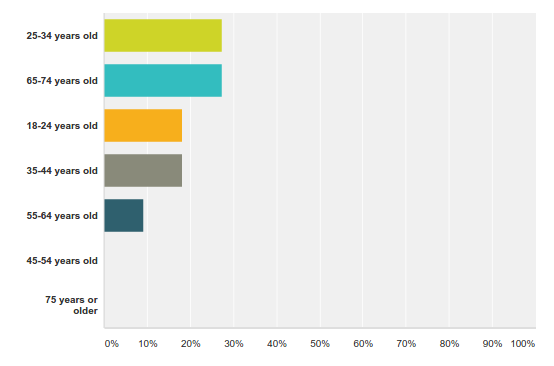
\includegraphics[scale=1]{images/ages_survey.png}
\end{adjustbox}
  \caption[Survey respondents ages ]{Survey respondents ages}
  \label{fig:survey_ages}
\end{figure}

Regarding the previous usage of air quality sources, only half of the pollution-sensitive respondents were able to name the websites or applications they were currently using, while all the non-sensitive respondents named at least one source of information. Also, the sensitive respondents who reported the use of air quality sources tended to use them on a more regular basis than non-sensitive users. Reflecting on these answers: sensitive users may be inclined to require a support tool on a regular basis, but not all of them are aware of their existence or does not feel the current sources meet their needs. 

The main findings from the survey were the potential new functionalities that users would like in a new Air Quality application; suggesting that there are unaddressed needs from current AQ sources. These are the main focus of the development of a new AQ application. From the \ref{fig:survey_new_features} we can see that the most important need is to visualise different individual pollutants, as current approaches often fail on treating them individually to enable decisions based on individual readings. The second most important unaddressed need is to be able to personalise the air quality advice given their personal circumstances. The third most important requirement is to compare and visualise individual pollutants over different periods of time. 

Another interesting outcome was whether including tools that would allow the users to keep track of their symptoms would be of interest. Just three of the eleven queried persons responded positively. Suggesting that they may feel unnecessary or tedious to input their symptoms data on a regular basis.


\begin{figure}[H]
\begin{adjustbox}{width=1\textwidth,center=\textwidth}
  \centering
  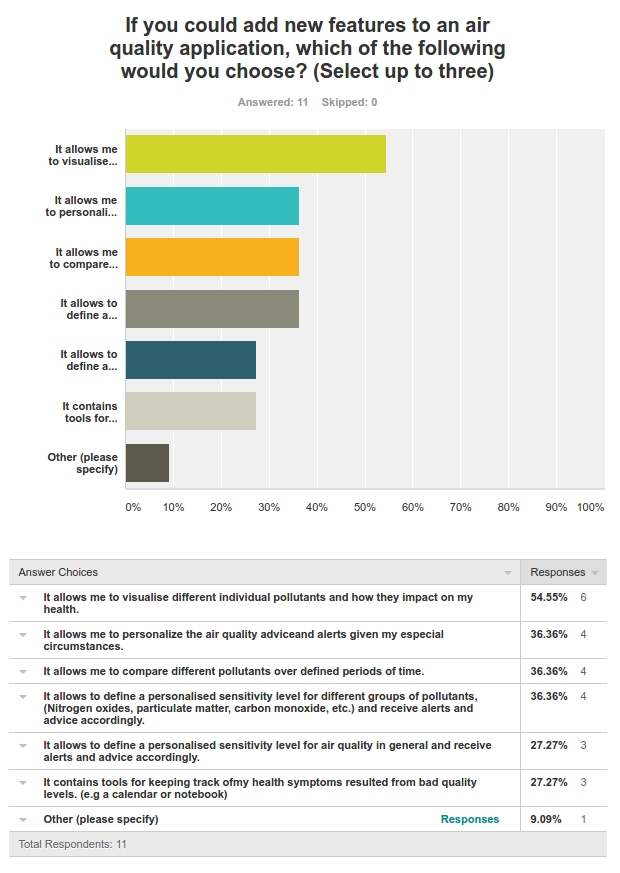
\includegraphics[scale=1]{images/new_features.png}
\end{adjustbox}
  \caption[New features for an AQ application]{New features for an AQ application}
  \label{fig:survey_new_features}
\end{figure}

\subsection{Interviews}

Meetings were held with the aforementioned researchers and domain experts to receive input from different points of view. At an early stage of the design, the first person who showed interest was Mic Starbuck. From his perspective as a person suffering from asthma he mentioned the need for a tool to be able to visualise the relative impact upon a person's health given different factors: like a person's health status, location, altitude, and individual pollutants. He mentioned as well that he browsed the web frequently to understand how the AQ is behaving at different points of the day to decide whether or not going outside or perform certain activities. 

Later on, the Asthma UK Center for Applied Research showed interest and a meeting was arranged. It took place with Dr Aziz Sheikh, Lynn, Morrice, Dr Soyiri Ireneous and Catherine Magill. They showed a favourable interest in collaborating with this project as well as participating closely to the School of Informatics in future research. They were presented with mock-ups as ideas for an application that would accomplish visualisation and tracking purposes. Visualisations from the need previously pointed out by Mic Starbuck, and tracking from the need from asthma sufferers to manage their illness by keeping their digital diary of symptoms and pollution spikes to be able to take better informed choices related to their health. However based on previous work on tracking asthma status they pointed out that applications that rely on user input should take into further consideration the particular context of the user to succeed. For instance, much effort would be required to develop interfaces suited for different types of users. Because of this more focus was paid in the visualisation and recommendation capabilities than the tracking capabilities.

Another meeting was held with Dr Soyiri Ireneous whose main research is in asthma, and Catherine Magill. The purpose of this session was to understand more in-depth the consequences of air pollution upon a person's health and how they might be presented in an air quality application. The possibility to include health advice was discussed, as data that is accompanied with an easy to follow advice is more valuable than data alone because the user can immediately know what to do under special circumstances. Also, Dr Soyiri as a mobile phone user was concerned is concerned with the speed of the applications he installs, as well the memory and battery usage.

\subsection{Functional requirements}

Because the time was limited; the development covered the first three and most important needs given by the final users as illustrated in the past section. The following list summarises the final formal functional requirements for the development:

\begin{itemize}
    \item Being able to visualise the air quality status in general.
    \item Being able to visualise individual pollutants status and information on how the impact on a person's health.
    \item Being able to visualise individual pollutants over time.
    \item Being able to receive advice about the air pollution based on the variables known by the application. That is the user location, age and pollution sensitivity. 
    \item Being able to personalise the received advice indicating the personal pollution tolerance or sensitivity.
\end{itemize}

\subsection{Non functional requirements}

Summarising from the meetings, the following was established as non-functional requirements:

\begin{itemize}
    \item Is adequate for mobile devices (\textbf{Mobility}).
    \begin{itemize}
        \item Does not consume much storage space.
        \item Does not consume much battery.
        \item Is compatible with multiple devices.
    \end{itemize}
    \item Is usable (\textbf{Usability}):
    \begin{itemize}
        \item Easy to learn.
        \item Attractive to use.
    \end{itemize}
    \item Is efficient (\textbf{Performance}).
    \begin{itemize}
        \item Starts rapidly
        \item Loads and displays visualizations fast
    \end{itemize}
\end{itemize}


\section{System architecture}
In order to accomplish the requirements, it is important to consider design choices that could add towards qualities that are more adequate for this kind of development. For this, a trade-off between the three qualities of the software will be considered as shown in Figure \ref{fig:balance_attributes}, since it is not always possible to have everything in a system because some attributes may be in conflict. For example, doing an extremely animated and attractive design would affect the performance of the system and its capability in accomplishing the primary goal. Architectural choices will be taking into account this trade-off.


\begin{figure}[H]
\begin{adjustbox}{width=.5\textwidth,center=\textwidth}
  \centering
  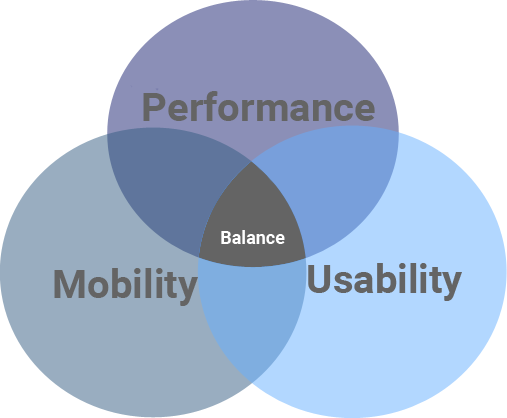
\includegraphics[scale=1]{images/balanceCircles.png}
\end{adjustbox}
  \caption[Finding a balance between software attributes]{Finding a balance between software attributes}
  \label{fig:balance_attributes}
\end{figure}

\subsection{Development approach and operating system}
It is possible that the development could take a hybrid or a native approach, as summarised in Table \ref{tab:development_approaches}. In a nutshell, it means that the software could be developed in a web-browser container and therefore be compatible with all devices able to display modern web-pages, or be developed using the native software development kit for each system (Android, iOS, etc) being only compatible with that specific operative system. A native development approach carries the disadvantage that new code would be needed for each operative system, but gaining many benefits, such as the response speed, being able to use advanced graphics and animation techniques and having an easy access to the native APIs and components of the device (e.g. GPS and gyroscope). In order to gain performance and usability a native approach has been chosen. Consequently, it is important to define the operating system target, which will solely be based on the market share of the most important operating systems according to IDC \footnote{\url{http://www.idc.com/prodserv/smartphone-os-market-share.jsp}}. Android holds an enormous share of 82.8\%, compared to 13.9\% of iOS, and 2.6\% for Windows phone (other systems just account for less than 1 percent of the market share.), because of this to target a wider range of mobile phone users the selected operative system is Android.

\begin{table}[ht]
\centering
\begin{adjustbox}{width=.6\textwidth,center=\textwidth}
\begin{tabular}{lrr}
  \hline
   - & Native & Hybrid  \\ \hline
   Language & Switf or Java & HTML and Javascript \\
   Speed & Fast & Medium \\
   Portability & None & High \\
   Advanced Graphics & High & Moderate \\
   Access to native APIs & High & Moderate \\
   Development cost & Expensive & Reasonable \\
   \hline
\end{tabular}
\end{adjustbox}
  \caption[Native vs hybrid development approach ]{Native vs hybrid development approach. (Adapted) \footnotemark }
\label{tab:development_approaches}
\end{table} 
\footnotetext{\url{http://julyrapid.com/hybrid-vs-native-mobile-app-decide-5-minutes/}}

\subsection{Air quality data source}
It was considered to acquire personal air quality sensors to provide real-time high-resolution data to the system; unfortunately, such devices are still not very feasible as they are costly and become obsolete over time due to loose of accuracy. One example is the Libelium Gases PRO sensor, which costs around \euro{}2000 and has an approximate lifetime of 12 months\footnote{\url{http://www.libelium.com/calibrated-air-quality-gas-dust-particle-matter-pm10-smart-cities/}}. 

As mentioned in the background section there are currently many fixed sensors around Scotland which include different measures depending on the type of the sensor. However, the data sensed by this devices is not exposed through any public API from the Scottish government, but as plain HTML web-pages. One possibility as well is using any third party air quality data source; such as the Breezometer air quality API\footnote{\url{https://breezometer.com/air-quality-api/overview/}} or the OpenAQ API\footnote{\url{https://openaq.org/#/}}. The first one is a private source of air quality data which bills for the queries to the service and may become not very cost-effective, the second is a public API source, but the number of sensors from each city in Scotland are limited compared to the official government sources. An example of this is the city of Glasgow, which from the official sources has 26 fixed sensors and from the public API only 4 are available. Because of this, to have a more accurate air quality source the data will be collected from the official sources and exposed to later query from the device. 

Missing this: (REF)
http://www.scottishairquality.co.uk/data/

\subsection{Infrastructure as a service}
IaaS or Infrastructure as a service is a cloud service that provides computing infrastructure on demand. The benefits of using such service as opposed to a traditional approaches are various. First, there is no need to buy, install and maintain a server on a fixed location, reducing the associated costs. Second, setting up an IaaS can be done within minutes, saving precious development time. The following options were considered for setting up an IaaS: 

\begin{itemize}
	\item Google Cloud platform \footnote{\url{https://cloud.google.com/}}
    \item Amazon Web Services \footnote{\url{https://aws.amazon.com/}}
    \item Microsoft Azure \footnote{\url{https://azure.microsoft.com/en-us/}}
\end{itemize}

Because of budget constraints, the most cost-effective solution was chosen, being Amazon's free tier the most generous allowing up to 12 month of free usage, as opposed to Microsoft's 30 days trial and Google's 60 days trial.

\subsection{Back-end technological choices}
The back end component of the system will perform 2 functions: Gather the required air quality data and insert it into a database; and provide service to the mobile application. For the  first function the easiest way to do it is via any available web-crawling libraries, such as Jspider\footnote{\url{http://j-spider.sourceforge.net/}} for Java or Scrapy \footnote{\url{http://scrapy.org/}} for Python. Scrapy was chosen because it is a complete and stable framework that can handle the crawling operations in an easy way. 
For the second component there is a need for a more robust component which can handle multiple queries to the health advice presented in Android. Because of this, Java will be (PEND)

\subsection{Schema-free database}
There will be the need to store the air quality readings somewhere to later query from the device. For this, there is the option to use standard SQL databases or schema-free databases. Analyzing the data that will be stored in further detail it will contain the readings gathered from each sensor in Scotland, and specific information such as their name, location and type of sensor. It is simple enough to be inserted without needing any relational schema . Moreover, the transactions between the devices and the database should be as fast as possible; without caring to much for instant reliability (because the sensors are updated at the soonest each hour). Taking into account these factors, it is more suitable the usage of a schema free database or NoSQL, specifically, it will be used a Dynamo NoSQL from the same Amazon Web Services infrastructure because it integrates easily with the already chosen IaaS. 

\subsection{Overall design}
The overall design of the infrastructure will be as shown in Figure \ref{fig:architecture}. The back-end and the database components will be running in Amazon Web Services, and the Android device will make use of the AWS SDK to make queries to the Dynamo database, and REST services to query the advice server running on Java. (PEND explain more?)

\begin{figure}[H]
\begin{adjustbox}{width=.8\textwidth,center=\textwidth}
  \centering
  \includegraphics[scale=1]{images/architecture.png}
\end{adjustbox}
  \caption[Architecture design]{Architecture design}
  \label{fig:architecture}
\end{figure}

\section{Mobile application}
The Android application will be the visible interface for the final user. At this point it is pertinent to understand the design choices that can affect our main quality attributes. The design of the user interface and the lower-level issues related to the management of the screen components. 

\subsection{User interface}
Three distinct screens will accomplish the functional requirements as shown in Figure \ref{fig:chain_of_screens}. The first screen will be responsible for displaying a general overview and the personalised advice, the second screen will show individual pollutants, and the third screen will show individual pollutants over time. There will be another introductory screen to allow users to input the personal details needed for the application.

One useful guideline at the design level to connect the screen between each other is simplicity. Having many different screens that accomplish many different purposes could result in overwhelming the user, because of this, the screens will be accessible at every time using a tabbed menu and enabling gestures to navigate through them. That is, the screens will become active by selecting a tab, or by swiping between them.


\begin{figure}[H]
\begin{adjustbox}{width=.45\textwidth,center=\textwidth}
  \centering
  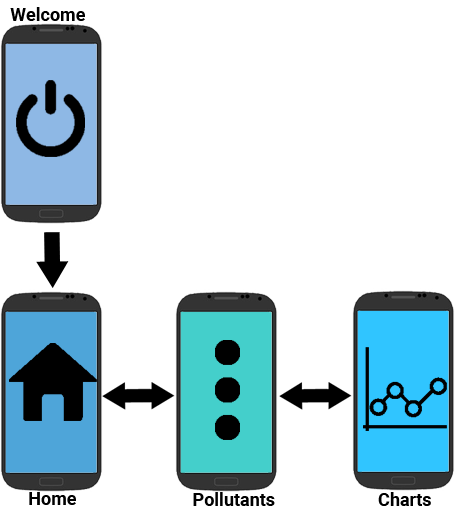
\includegraphics[scale=1]{images/screenChain.png}
\end{adjustbox}
  \caption[Chain of screens]{Chain of screens}
  \label{fig:chain_of_screens}
\end{figure}

\subsection{Activities}
The former screens will be developed individually by the use of activities. An Activity is the abstraction used by the Android framework to contain the visual and run-time elements of the currently displayed screen. The way Activities are created and maintained in the screen is quite unusual in contrast with standard Java Swing interfaces. It makes use of an event driven life-cycle that must be understood ahead to achieve an smooth and error-free behavior. 

Because the available RAM is limited on a handheld device and it has to be shared with all other running applications, it is not possible to maintain  all activities instances in memory. The activities lifecycle is a workaround for this problem, allowing the Dalvik virtual machine (A virtual machine that runs all Android programs) to automatically determine which activities will be kept in memory. Therefore, it is unknown the time it will be requested to start-up resume or stop and all possible precautions should be taken for it to keep working from any call point .

The lifecycle is illustrated in Figure \ref{fig:activities_lifecycle}. It can be observed that the first method called by Android is the \textit{onCreate()} method, used to instantiate the requested activity and any screen components. Later on, the application can pass to other states until it is stopped and started again from a different entry point to the one it was previously created from. The activities should be able to handle both starting points and restore any state left by the user when the activity was requested to stop. 

\begin{figure}[H]
\begin{adjustbox}{width=1\textwidth,center=\textwidth}
  \centering
  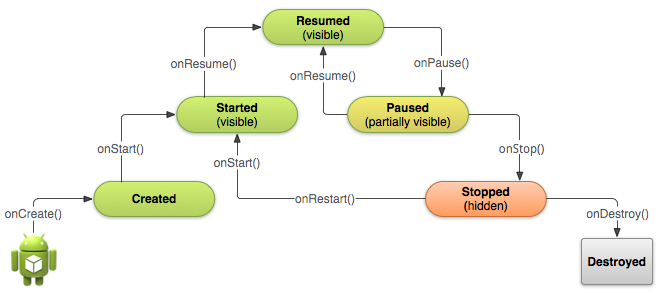
\includegraphics[scale=1]{images/basic-lifecycle.png}
\end{adjustbox}
  \caption[Android activities lifecycle]{Android activities lifecycle\footnotemark}
  \label{fig:activities_lifecycle}
\end{figure}
\footnotetext{\url{https://developer.android.com/training/basics/activity-lifecycle/starting.html}}

\subsection{Layouts}
The main component to render a screen in Android is the Layout. Layouts make use of XML to define the objects in the screen as shown in the example bellow, which renders a \textit{TextView} object followed by a \textit{Button} object. Layouts need to be attached to an activity or fragment to give them behaviour. Once attached, the components defined by the layout can be extracted by using their id's and the method \textit{findViewByID}
\begin{verbatim}
<?xml version="1.0" encoding="utf-8"?>
<LinearLayout xmlns:android="http://schemas.android.com/apk/res/android"
              android:layout_width="match_parent"
              android:layout_height="match_parent"
              android:orientation="vertical" >
    <TextView android:id="@+id/text"
              android:layout_width="wrap_content"
              android:layout_height="wrap_content"
              android:text="Text" />
    <Button android:id="@+id/button"
            android:layout_width="wrap_content"
            android:layout_height="wrap_content"
            android:text="Text" />
</LinearLayout>
\end{verbatim}

It is important to understand the correct coupling of Android layouts because this influences how fast the screen is rendered. The rendering process is called \textit{inflating} and occurs in the \textit{onCreate()} method. As the activities are rendered on the screen children components are attached and may call to render their own layout and so on, potentially slowing down the the application. For this purpose, the Android SDK makes available the Android device monitor that can be employed to understand how much time is taking to render all the components displayed at a given time. 

The Android device monitor helps to visualise the components that are taking part of the screen at some point in run-time. It shows from the top most element (the root) to the bottom most element (the leaf) how they are attached together and which element of the entire tree is taking the most time to render, helping in the debugging process. As shown in Figure \ref{fig:android_device_monitor} the delaying components are marked with red dots; wich means that the rendering of that specific screen component is among the slowest half of views, the yellow means the view renders faster than the bottom half of the other views and the green means that renders faster than at least half of the other views. The understanding of this tool is important in order to achieve the required performance quality attribute. 

\begin{figure}[H]
\begin{adjustbox}{width=1\textwidth,center=\textwidth}
  \centering
  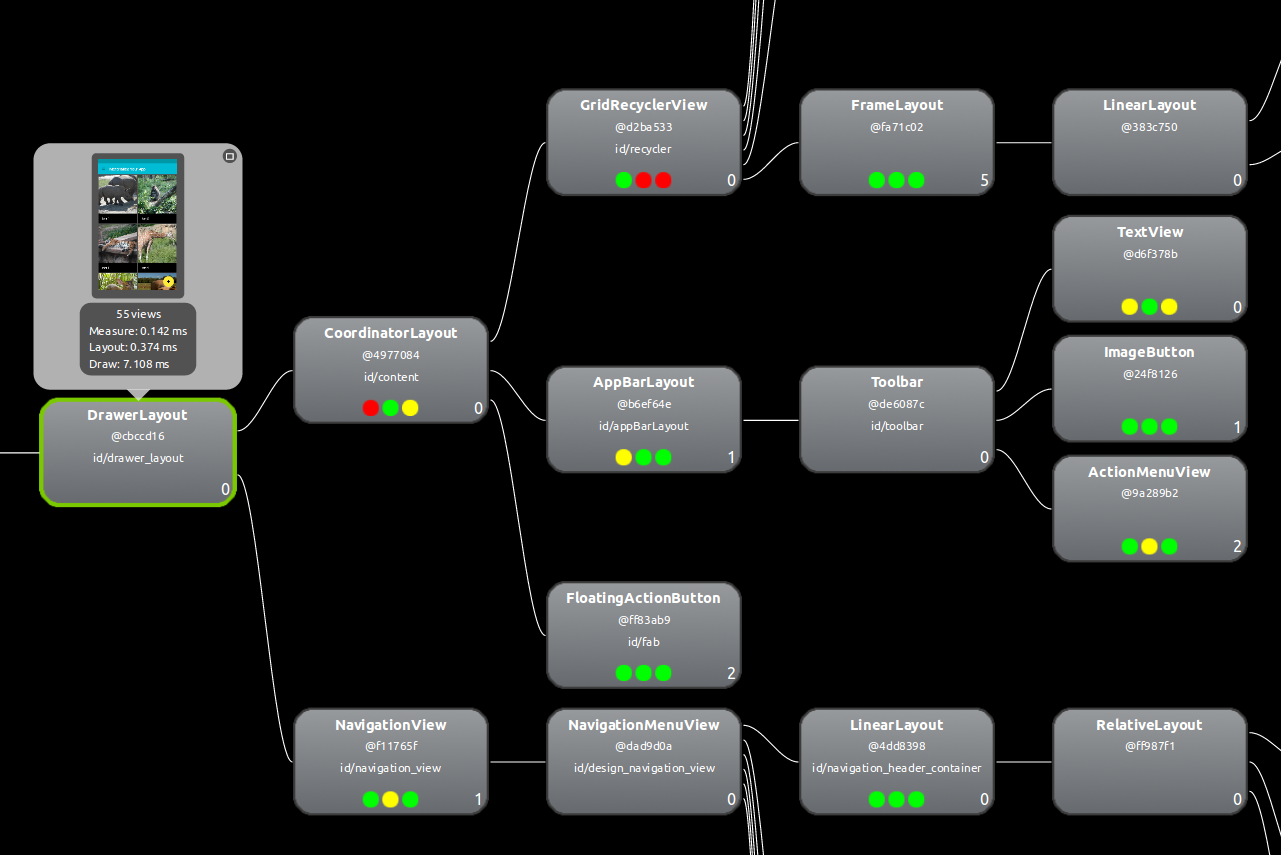
\includegraphics[scale=1]{images/android_device_monitor_2.png}
\end{adjustbox}
  \caption[Android device monitor]{Android device monitor.}
  \label{fig:android_device_monitor}
\end{figure}

\subsection{Material design}
As well as understanding how to achieve an smooth behavior within the application is wise to revise how to make good use of the design principles available to enhance usability and its implied attributes: ease of use and attractiveness. 

According to Google: \begin{displayquote}Material design is  a visual language for our users that synthesizes the classic principles of good design with the innovation and possibility of technology and science. \end{displayquote} 

The material design framework helps with principles that address design issues to allow every application user to navigate, understand and use the designed user interface (UI) successfully. It also serves to unify the experience across different devices and screen sizes, so that users that are used to applications in general; will be able to understand in a natural way design cues of new applications. The following principles are adhered:   

\begin{itemize}
	\item Material: The material metaphor is based on paper and ink as in the real world, in three dimensions using lights and shadows. The intention is to close the gap between the perception of real world elements and digital elements. 
    \item Graphics: The use of graphical elements such as typographies, icons, adequate colors and images make up a pleasant interface and give hierarchy and meaning. 
    \item Motion: User actions that initiate motion and transform the state of the interface serve as playful cues that help to understand the flow of the interface as well as to provide continuity and feedback. 
\end{itemize}


\begin{figure}[H]
\begin{adjustbox}{width=1\textwidth,center=\textwidth}
  \centering
  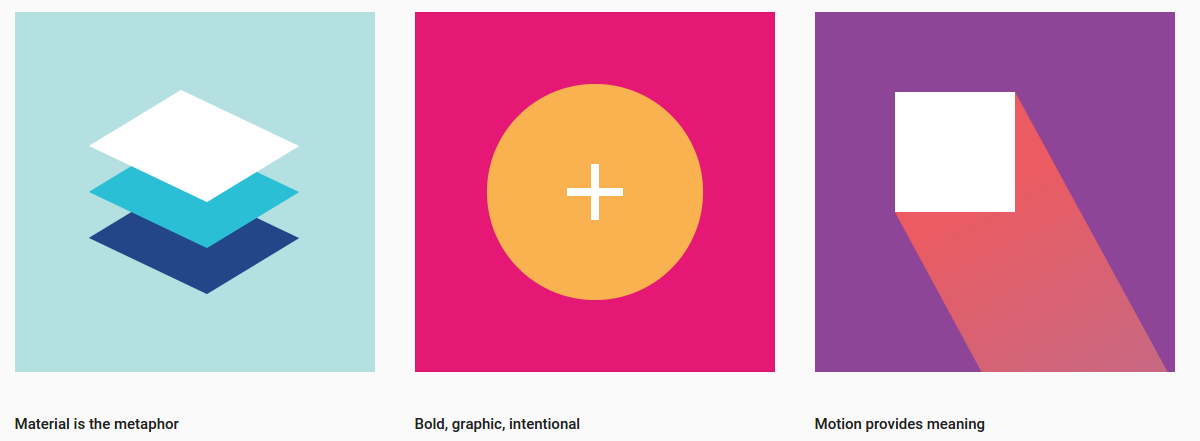
\includegraphics[scale=1]{images/material_google.png}
\end{adjustbox}
  \caption[Material design framework]{Material design framework \footnotemark}
  \label{fig:android_material_design}
\end{figure}
\footnotetext{\url{https://material.google.com/}}

\subsection{Targeted devices}
As the android OS and APIs (Aplication Programming Interfaces) are updated over time; some applications built with later SDK's versions will not be compatible with earlier OS' versions. Because of this, it is important to define the earliest operative system that will be included in the development. For this, considerations such as the number of users that are still using old versions of android and new features that might be useful from newer SDK versions should be studied. For instance, the most used OS distribution nowadays is KitKat which makes use of an API level 19 as shown in Figure \ref{fig:android_platform_versions}.  Unfortunately, it does not offer native support for material elements, which are a strong positive for this development. A workaround for this problem is to include the Android support library\footnote{\url{https://developer.android.com/topic/libraries/support-library/index.html}} which will provide compatibility for features made available in newer versions of Android. The final targeted API is level 19 (KitKat) to use an up to date stable API and to include up to the 79\% of the Android users.  

\begin{figure}[H]
\begin{adjustbox}{width=1\textwidth,center=\textwidth}
  \centering
  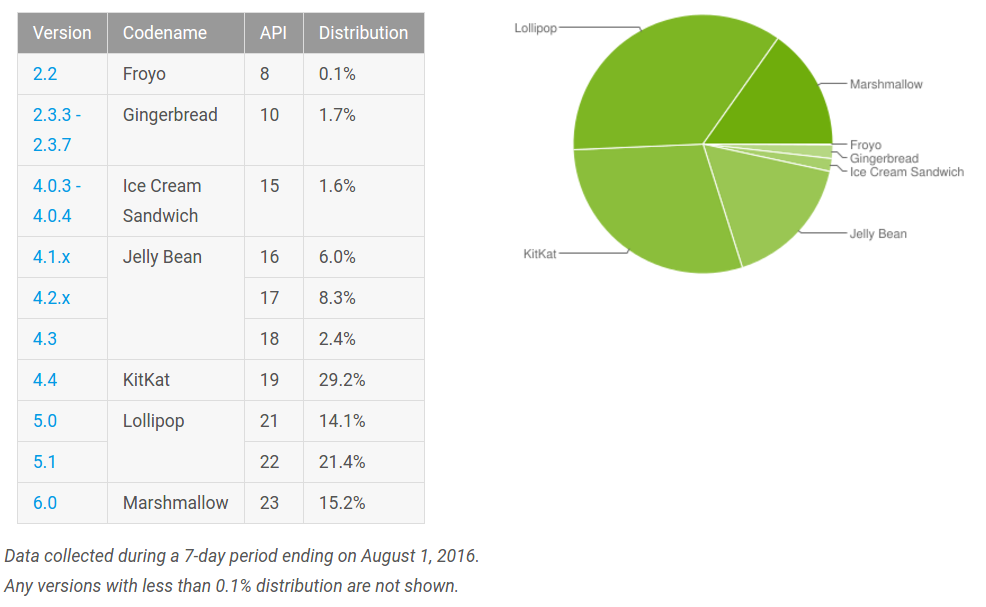
\includegraphics[scale=1]{images/android_platform_versions.png}
\end{adjustbox}
  \caption[Devices running a given version of Android]{Devices running a given version of Android \footnotemark}
\end{figure}
\footnotetext{\url{https://developer.android.com/about/dashboards/index.html}}

\section{Back-end}
More in detail, the back-end architecture will be composed as shown in Figure \ref{fig:architecture_back_end_detail}. A virtual machine will run Ubuntu Linux because it is a very stable and compatible version of Linux. There was also a possibility to use a custom amazon flavor of Linux, which was not viable due software compatibility issues. The back-end will host two main components to power the application, the data service and the advice service. 

\begin{figure}[H]
\begin{adjustbox}{width=.6\textwidth,center=\textwidth}
  \centering
  \includegraphics[scale=1]{images/architecture_back_end_detail.png}
\end{adjustbox}
  \caption[Back-end architecture]{Back-end architecture detail}
  \label{fig:architecture_back_end_detail}
\end{figure}


\subsection{Data Service}

 The air data source is the air quality in Scotland website. Because it displays the updated readings in HTML, a web crawler is needed to navigate the readings making use of XPATH selectors to extract the required data. Once extracted, they will be inserted in JSON format directly to the dynamo database.
 
A daemon is a program that runs in the background autonomously, this daemon will call the web crawler every half hour to get the most up-to date readings from the air quality readings (They are updated at most each hour). 

\subsection{Advice Service}
The advice service will be responsible to provide health advice based on the CMEAP\cite{HealthProtectionAgencyfortheCommitteeontheMedicalEffectsofAirPollutants2011}. Before analyzing the techniques that can be considered to translate the advice from the CMEAP into a service, there are few things to notice. The document has different categories of advice based on the sensitivity and age of the persons, they are not simple data statements that can be easily used from a database, but more of logical statements. Also, it is likely that the health statements would need to be modified or expanded in the future. 

When it comes to provide logic or 'intelligence' to a system for it to take choices (like the ones that are needed for the health advice) there are two general approaches that may be taken. Rule based systems and machine learning techniques. Rule based systems or expert systems are a good fit when all the options for the system are known beforehand; and when all the conditions can be easily written as \textit{if else statements}. On the other hand; machine learning techniques are useful when the datasets are fairly large and the rules have to be made at execution time. Because of this, the easiest way to provide the system the capability to give the required health advice given the user's personal circumstances is via an expert system.

\section{First prototype}
Following the sketched application design and the interaction design methodology, the first prototype was drawn in order to accomplish the user requirements and to start defining how the final interface would look like. As mentioned, the application would be composed of three final distinct visualizations that will achieve the main functional requirements:

\begin{itemize}
	\item Visualize current air quality and provide health advice.
    \item Visualize individual pollutants status and information about their sources and effects.
    \item Visualize individual pollutants over time.
\end{itemize}


\begin{figure}[H]
\begin{adjustbox}{width=1.2\textwidth,center=\textwidth}
  \centering
  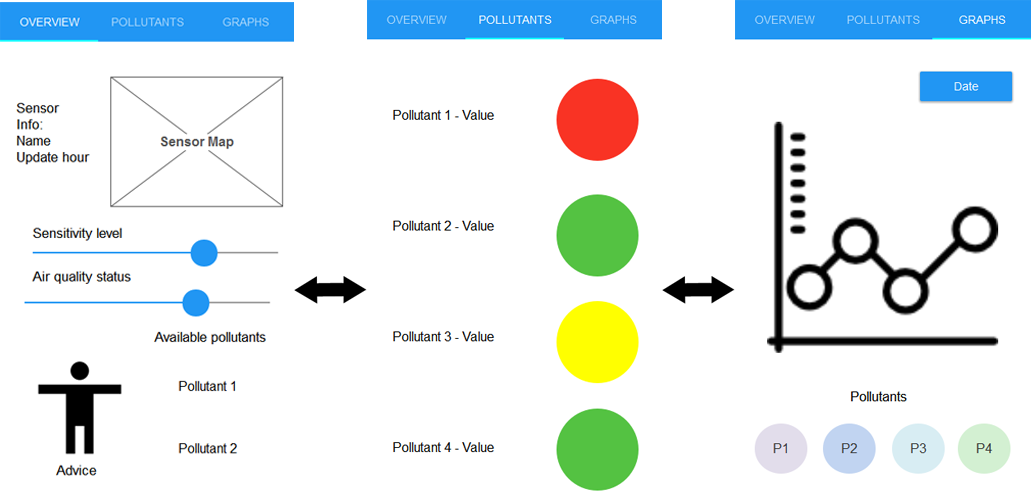
\includegraphics[scale=1]{images/firstPrototype.png}
\end{adjustbox}
  \caption[Frist prototype]{First prototype. From left to right: first, second and third visualization.}
  \label{fig:first_visualization_first_prototype}
\end{figure}


\subsection{First visualization}

The first visualization would contain firsthand pertinent information that would accomplish different functions: letting know in an understandable, visual way the current air quality status and its components, providing information about the source of the air quality reading, showing the air quality advice given the user configuration and let the user configure the air quality advice in a playful way. We could think of this screen as a dashboard that will give the user the required basic information to use the rest of the application, in fact; the displayed by this screen is enough to get a full picture of what is going on without much detail.

This screen is composed as shown in Figure \ref{fig:first_visualization_first_prototype}. It is visually divided into the top and bottom component. The top component is information about the sensor to provide the user confidence about the reading by means of a map, the hour it was last updated, and the name location of the sensor. The bottom component contains two bars: one for adjusting the sensitivity level, and the other one to show the air quality status followed by the health advice in text and the pollutants that are taking part of the reading at the point it was taken. 

\subsection{Second visualization}

The second visualizations aims to provide an individual visual hint for each pollutant. The need for this visualization arises from the difficulty to observe how the readings are at a pollutant level without expert understanding of air quality regulations. The overall idea is to show a list of the pollutants that are present at the moment with a visual cue to allow an immediate insight of the reading as well as containing the official measure and the measurement unit. Also, by clicking in each pollutant it will be possible to examine more specific information about the pollutant.

\subsection{Third visualization}

The final visualization will provide the full detail of how the readings were behaving through the day, or in a specific date. The need for this visualization arose from the need by sensitive persons to relate their symptoms to pollution spikes in order to gain knowledge about what might be affecting them at a pollutant level and enable them for better decision support based on this knowledge. For this purpose, a line graph is employed as is the most adequate tool to show readings over time. Also, the same pollutants that were taking part of the first and second visualizations will be consistent in this screen. The difference is that they will be touch-enabled to allow the user to select which  pollutant to visualize as a way of providing interaction and control over the interface to the user. At the top of the screen will be located controls to define the specific date and time of the readings. 

\chapter{Design}
\section{Design goals}
\subsection{Trade-off}
\section{Front end}
\section{Back end}
\chapter{Implementation}
Before being able to develop a second working prototype that implements some of the functionality it is needed a fully functional back-end component. This chapter describes how this was was achieved with the elected design and technological choices going from the development of each back-end component to the development and implementation of a second and a third prototype.
\section{Back-end implementation}

\iffalse
\subsection{Environment setup}
Following the design and technological choices from the previous chapter; the dedicated hardware components were launched from Amazon Web Services. 
\fi


\subsection{Database}
Dynamo was the chosen database as justified in the design chapter. It is a schema-free database that only requires a table name and a primary key. The primary key can be composed of up to two attributes, in which case the the first attribute defines the partition range and the second attribute defines the sorting over that partition. Dynamo is extremely efficient when used in the correct way. 

Designing the table to contain the air quality readings is straightforward. The key is composed by the unique ID of the fixed sensor being the partition key, and the updated hour being the partition sort key. This provides the advantage that all the readings of an specific sensor can be retrieved together, and that they will be dispatched sorted, saving computing time on the client. Other general usage tables are also created to contain the coordinates of all sensors, and the COMEAP thresholds for each pollutant. These tables contain at most 20 items and are designed to be retrieved as a whole, so there is no need to sort them on a second attribute.

\subsection{Web crawler and daemon}
A web crawler is a service that automatically browses the web and extracts useful information to later insert it into a persistent storage. The air quality data needed to feed the application will be extracted from the Air Quality in Scotland website (REF) using scrappy as discussed in previous chapters. The way scrappy extracts structured data from a web-page is by browsing the HTML document with XPATH expressions. 

\begin{figure}[H]
\begin{adjustbox}{width=.5\textwidth,center=\textwidth}
  \centering
  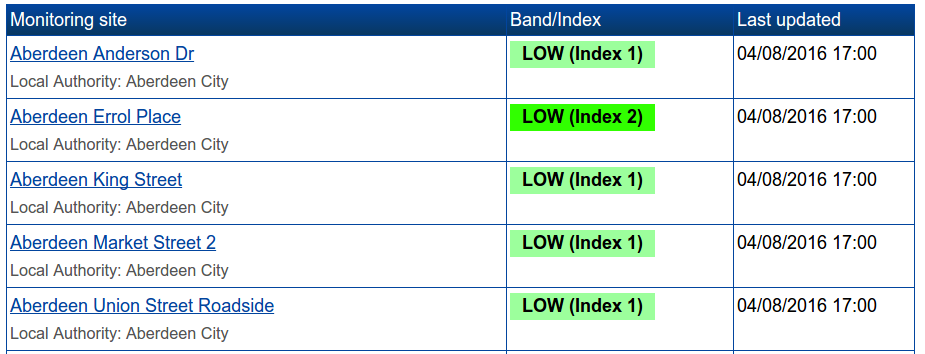
\includegraphics[scale=1]{images/monitoring_summary.png}
\end{adjustbox}
  \caption[Pollution sensors list]{Pollution sensors list \footnotemark}
  \label{fig:pollution_sensors_list}
\end{figure}
\footnotetext{\url{http://www.scottishairquality.co.uk/latest/summary}}

The website data source contains many sensors from different authorities in Scotland as shown in Figure \ref{fig:pollution_sensors_list}, they aggregate the data and display a list of the available sensors. The first thing the crawler would need to do is to extract the links to navigate through all the available sensors. The rendered sensor list table looks like the code bellow in plain HTML. It is noticeable that the XPATH selector needs to go through the table to reach the \textit{href} attribute in order to access the data for that specific sensor. 

To select the \textit{href} attribute: \bigskip

{\centering
\begin{BVerbatim}
//tr/td[1]/a@href
\end{BVerbatim}
\par
}\bigskip

The output of the XPATH selector is highlighted in red: 

\begin{Verbatim}[fontsize=\small,commandchars=\\\(\)]
<table>
  <tbody>
    <tr>
      <td><a href="(\color(red)site-info?site_id=ABD1")>Aberdeen Anderson Dr</a><br></td>
      <td><span>LOW (Index 1)</span></td>
    </tr>
      <tr>
      <td><a href="(\color(red)site-info?site_id=ABD)">Aberdeen Errol Place</a><br></td>
      <td><span>LOW (Index 2)</span></td>
    </tr>
  </tbody>
</table>
\end{Verbatim}

Once that the URL containing the data is extracted, scrappy executes another request to select the interesting data for each sensor. The readings are rendered through a table which contains the pollutant, the band, the concentration and the update period as shown in Figure \ref{fig:pollution_site readings}

\begin{figure}[H]
\begin{adjustbox}{width=.5\textwidth,center=\textwidth}
  \centering
  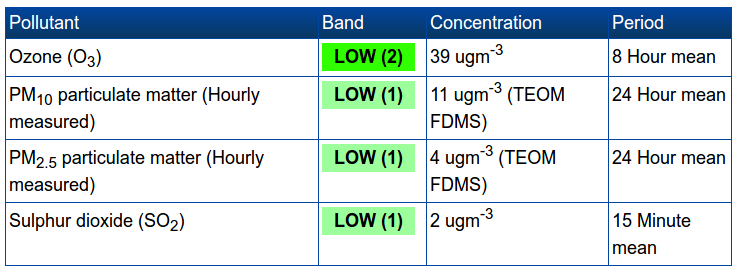
\includegraphics[scale=1]{images/site_readings.png}
\end{adjustbox}
  \caption[Edinburgh St Leonard's site readings]{Edinburgh St Leonard's site readings \footnotemark}
  \label{fig:pollution_site readings}
\end{figure}
\footnotetext{\url{http://www.scottishairquality.co.uk/latest/site-info?site_id=ED3}}

To extract the pollutants information contained in the the table all the \textit{td} elements are selected: 

{\centering
\begin{BVerbatim}
td[1]
\end{BVerbatim}
\par
}\bigskip

The output of the XPATH selector is highlighted in red: 

\begin{Verbatim}[fontsize=\small,commandchars=\\\(\)]
<table>
  <tbody>
    <tr>
      <td>(\color(red)Ozone (O<sub>3</sub>))</td>
      <td>(\color(red)LOW (2))</td>
      <td>(\color(red)39 ugm<sup>-3)</sup></td>
      <td>(\color(red)8 Hour mean)</td>
    </tr>
  <tr>
    <td>(\color(red)PM<sub>10</sub> particulate matter (Hourly measured))</td>
    <td>(\color(red)LOW (1))</td>
    <td>(\color(red)11 ugm<sup>-3</sup> (TEOM FDMS))</td>
    <td>(\color(red)24 Hour mean)</td>
  </tbody>
</table>                
\end{Verbatim}

Following the same principle the remaining meta-data such as the reading time-stamp and the sensor details are extracted. Still, the data data is not in the optimal format yet, some readings contain embedded HTML tags that need to be cleaned before any insertion in the database. Fortunately, scrappy provides a pipeline process before exporting the data into the desired format. The cleaning process is straightforward, by cropping the undesired tags with python strings processing. 

Once the data is ready to be exported, it is translated into a python \textit{dict} and inserted right-away in the dynamo table: \bigskip

{\centering
\begin{BVerbatim}
        table.put_item(Item = dict(sensor_reading))
\end{BVerbatim}
\par
}\bigskip


The described above python script will be executed constantly to keep the data as up to date as possible. Unix systems have a built-in daemon utility that can be used to execute the script directly called cron. This service reads a crontab file containing the information of the all the scheduled tasks. In order to add an entry to the crontab file and indicate that the the crawler script will be executed every 30 minutes, the following command is executed: \bigskip

{\centering
\begin{BVerbatim}
        */30 * * * * python crawler.py
\end{BVerbatim}
\par
}

\subsection{Advice service}
The advice service will respond the requests from the android device to provide the personalized health advice as discussed in previous chapters. It is composed of two components: an expert system and a java servlet to expose the service through HTTP GET requests. 

The first task is to translate the advice offered by the CMEAP into rules to form a knowledge base. This knowledge base will live in the memory of the java web container and whenever it receives new queries it will infer the advice form the asserted facts. The facts representing the advice are like \textit{if-else} statements that focus on three conditions: the pollution level index, the sensitivity of the person and the age of the person. 

The Jess engine allows to define templates, which are like java classes that describe how a statement should look like when asserted. The actual values contained by the fact are named slots. These templates are useful to describe the conditions that are needed to assert an advice. For instance, the templates \textit{pollutionLevel} and \textit{person} can be defined in the following way: 

{\centering
\begin{spverbatim}
(deftemplate pollutionLevel
    (slot value)
)

(deftemplate person
    (slot age)
    (slot sensitivity); The possible values are 1 and 2.
)
\end{spverbatim}
\par
}

The logic in Jess is modeled with rules. They define the conditions or facts that should be fulfilled in order to assert a new fact. The following rule is an example that models the CMEAP advice given to adult sensitive individuals when the air quality index is in a level between 4 and 6 points. If all these conditions are fulfilled then it is possible to assert the advice: "Consider reducing strenuous physical activity, particularly outdoors". 

{\centering
\begin{spverbatim}
(defrule consider_reducing_strenuous_activity_sensitive_4_6
    ?per <- (person {sensitivity >= 2})
    ?per <- (person {age >= 65})
    ?pol <- (pollutionLevel {value >= 4 && value <= 6})
    =>
    (assert
        (advice (text "Consider reducing strenuous physical activity, particularly outdoors")))
)
\end{spverbatim}
\par
}

The rule engine is initialized in the context of the java enterprise web container and the facts are loaded from a \textit{facts.clp} file to ease the way they can be later modified. 

To grant android access to the advice assertions, the inference engine was exposed in a public domain on the amazon infrastructure. The running servlet handles all incoming \textit{get} requests asking for the advice service. The client has to append the age, the sensitivity and the pollution level variables to the \textit{http get} request in the form of query parameters as in the following example: \bigskip


{\centering
\begin{BVerbatim}
http://.../Advice/advice?age=?&sensitivity=?&airQualityIndex=?
\end{BVerbatim}
\par
}

\section{Front-end implementation}
\subsection{Access to air quality data}
Once the services are available to query, the connection between the device and the air quality data hosted on dynamo has been implemented. Amazon makes available an android library ready to connect to the database readings\footnote{\url{https://aws.amazon.com/mobile/sdk/}}, it is included as a dependence within the android project. In order to handle and represent the database entries in android, Plain Old Java Objects \textit{POJO's} have been defined. They  are simple classes that describe the general structure and contents of a persisted data reading. An example is the following \textit{SensorReading}, which represents the raw \textit{JSON} database reading  and contains a list of the available pollutants, the date it was last updated, and the air quality index:

{\centering
\begin{spverbatim}

@DynamoDBTable(tableName = "airquality_readings")
public class SensorReading {

    private HashMap<String, Pollutant> pollutants = new HashMap<>();
    private String lastUpdated;
    private String airQualityIndex;
}
\end{spverbatim}
\par
}

This eases the way the data is queried from the device, allowing to define a \textit{DatabaseManager} to retrieve the readings in the following way: 

{\centering
\begin{spverbatim}
public List<SensorReading> getReadingsBySourceID(String sourceID, String since, String to) {

  Condition rangeKeyCondition = new Condition().
    withComparisonOperator(ComparisonOperator.BETWEEN.toString()).
    withAttributeValueList(new AttributeValue().
    withS(since), new AttributeValue().withS(to));

  DynamoDBQueryExpression<SensorReading> queryExpression = new
    DynamoDBQueryExpression().
    withHashKeyValues(sourceID).
    withRangeKeyCondition("lastUpdated", rangeKeyCondition);
  
return dynamoDBMapper.query(SensorReading.class, queryExpression);
}
\end{spverbatim}
\par
}

\subsection{Localizing the closest sensor reading}
Because many sensors may be available to query, the closest sensor should be identified and displayed. To provide localization features to the application it should inform that it has the intention to use such features before installed. To do so, the permission is added to the project \textit{manifest.xml} in the following way: \bigskip

{\centering
\begin{BVerbatim}
<uses-permission android:name="android.permission.ACCESS_COARSE_LOCATION"/>
\end{BVerbatim}
\par
}
\bigskip

Once that the location permissions have been granted, the application retrieves the last sensed location by the device and a list including all available sensors and their locations from the dynamo database. The task is to find out the closest sensor given the full coordinate list and the current location, which is also in longitude-latitude format. The closest sensor is chosen by calculating the distance between all options using the distance between two points formula: 

\begin{equation}
d={\sqrt {(\Delta x)^{2}+(\Delta y)^{2}}}={\sqrt {(x_{2}-x_{1})^{2}+(y_{2}-y_{1})^{2}}}.\,
\end{equation}

\subsection{Libraries and custom components}
Many android UI components like buttons, bars or windows are already built and made available for public usage. Because crafting all the interface components from scratch is an extensive time-consuming task, most UI components were be outsourced. Just in very specific cases where no component was found suitable, it was developed from scratch. 
The following public libraries were used to construct the UI:
\begin{itemize}
    \item Deco view charting \footnote{\url{https://github.com/bmarrdev/android-DecoView-charting}}: Provides components to create animated circular charts.
    \item MPAndroidChart \footnote{\url{https://github.com/PhilJay/MPAndroidChart}}: Provides components to create many different types of charts: lines bar and pie charts among others.
    \item Android simple tooltip \footnote{\url{https://github.com/douglasjunior/android-simple-tooltip}}: Provides a tool-tip component.
	\item Material date-time picker \footnote{\url{https://github.com/wdullaer/MaterialDateTimePicker}}: A built-in calendar to select time and date.
  \item Round corner progress bar \footnote{\url{https://github.com/akexorcist/Android-RoundCornerProgressBar}}: A fancy fully configurable progress bar.
\end{itemize}

\section{Second Prototype}
Now that the back-end is implemented to serve the application and that all the android components are in place, it is possible to describe a second prototype with some working capabilities, like retrieving and rendering real-data from the cloud services. This prototype will follow the established on previous chapters but providing a real interactive experience in order to get feedback from users and make improvements before releasing a third prototype. 

\begin{figure}[H]
\begin{adjustbox}{width=1.2\textwidth,center=\textwidth}
  \centering
  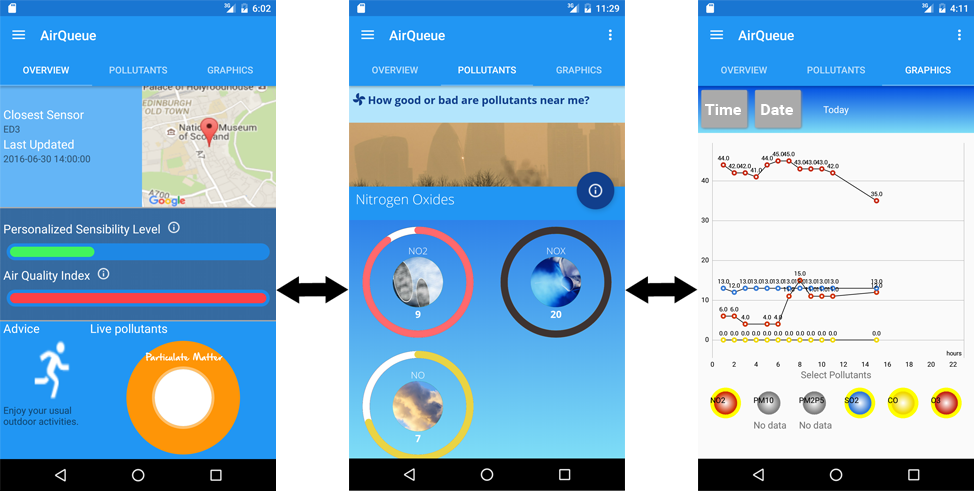
\includegraphics[scale=1]{images/secondPrototype.png}
\end{adjustbox}
  \caption[Second prototype]{Second prototype. From left to right: first, second and third visualization.}
  \label{fig:first_second_prototype}
\end{figure}

\subsection{First visualization}
At the top of the screen information of the air quality sensor is rendered employing text and a map. The map is retrieved by coordinates using the Google-maps API\footnote{\url{https://developers.google.com/maps/}}. In the center, there are two progress bars, one serves to adjust the personalized sensitivity level, and another one shows the current air quality index. The bottom components are including the personalized health advice, and the available pollutants at this time (In figure \ref{fig:first_second_prototype} the only pollutant available is particle matter). 

At this iteration the color choices are starting to be defined, yet they are not perfect but provide a guidance on what is wanted. The color that is desired to be predominant is blue, because it evokes to fresh air. There are separators within the screen to indicate that the sections accomplishes different functions and to guide the user through its learning. Also, the font choices pretend to provide understandable text. 

\subsection{Second visualization}
This visualization as previously stated aims to give an understandable first insight of the current pollution at a particle level. At this iteration is considered to include all particles in 'spheres' which contain the reading rendered in a circular graph that change in color and arc coverage according to the reading. The pollutants are grouped per category, in the Figure \ref{fig:first_second_prototype} are shown pollutants known as nitrogen oxides. Furthermore, images are included for the user to identify the current category and particle with ease.

To accomplish the second sub-requirement which is include further information about the pollutant when clicked, a second sub-screen was included. This one contains simple textual information about the pollutant sources and its associated health effects as shown in Figure \ref{fig:second_visualization_sub_screen}. 

\begin{figure}[H]
\begin{adjustbox}{width=.3\textwidth,center=\textwidth}
  \centering
  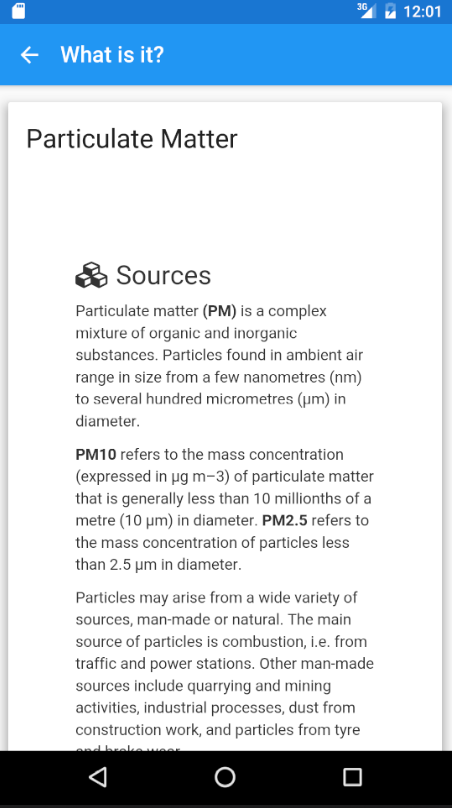
\includegraphics[scale=1]{images/second_visualization_sub_screen.png}
\end{adjustbox}
  \caption[Pollutant sources and effects screen]{Pollutant sources and effects screen}
  \label{fig:second_visualization_sub_screen}
\end{figure}

\subsection{Third visualization}
The third visualization includes the particles over defined periods of time using a line graph. The x axis represents the time while the y axis represents the reading. The user is able to select the data on specific dates and hours by using the available date and time buttons. At this iteration it was decided that the user would be able to overlap different pollutants and render them simultaneously on the same graph, this is done by selecting the pollutants on the bottom. Also, different colors are associated with the pollutants to be able to recognize them in the graph.

\section{Third prototype}
For the making of a third prototype, there were inner small evaluations with different users and stakeholders as mentioned in the Methodology section (REF). Their feedback was taken into account to discover what was failing with the second iteration and improve this final prototype. 

\begin{figure}[H]
\begin{adjustbox}{width=1.2\textwidth,center=\textwidth}
  \centering
  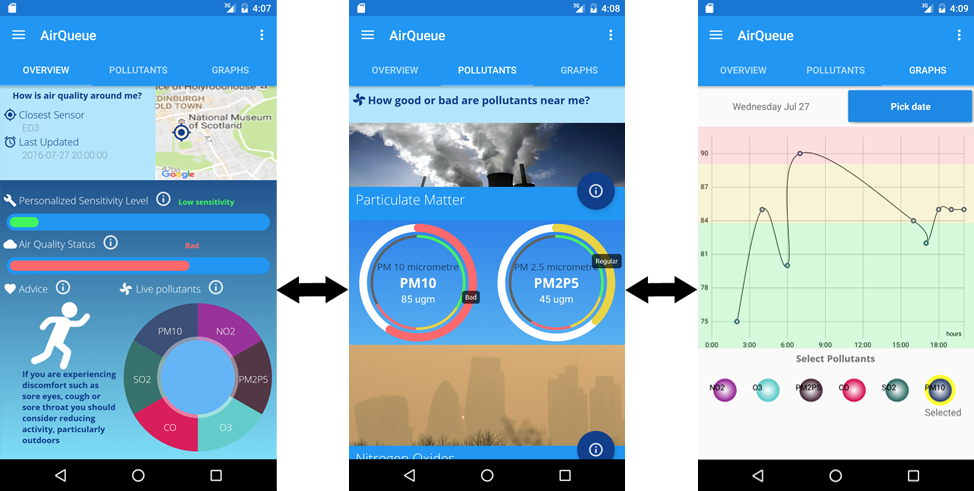
\includegraphics[scale=1]{images/thirdPrototype.png}
\end{adjustbox}
  \caption[Second visualization sub-screen]{Second visualization sub-screen.}
  \label{fig:third_prototype}
\end{figure}

\subsection{First visualization}
The findings from evaluating the second version of this screen were that the overall usability of the interface was not high nor low. People could use the interface after few attempts by playing around, but they were sometimes confused about what the elements were doing, and how to use them. Because of this the interface was improved to achieve a better learn-ability through changing the arrangement of the elements, the colors and adding other indicative visual and textual elements.
The improvements with respect the past iteration were the following:
\begin{itemize}
	\item  The way the interface is sectioned was changed. Having three sections was leading for confusion rather than for guidance.
    \item Background colors were changed to allow the components to be more distinguishable employing one main color in the top, and one gradient in the bottom.
    \item  The three three colors employed in this screen blend together better to avoid distracting the user.
    \item Indicative icons were added to provide usability. It is now easier to learn how to navigate through the interface.
    \item Info buttons with tool-tips were added. They give further information about what is happening with a particular screen component. For instance they say how to adjust the personalized sensitivity level, or where does the air quality status comes from. This to provide confidence. 
    \item Text fonts were richly improved, using the Google recommended fonts when appropriate:  Open-Sans and Robotto.
\end{itemize}

\subsection{Second visualization}
The second iteration of this screen was not very hard to use overall, the users were able to navigate through this interface with ease. On the other hand, feedback also showed that there were too many images leading to distraction. 

The improvements with respect the past iteration were the following:
\begin{itemize}
	\item The images on the center of each pollutant were confusing rather than accomplishing an associative function. They were removed.
    \item Apart from the associative colors in the circular graph (green, yellow, red) a textual tag was included (good, regular, bad).
    \item The titles of the pollutants were expanded, as they were not very distinguishable. 
    \item An inner smaller circle explaining the thresholds for each pollutant through traffic light colors was added to the circular graph. 
    \item Text fonts were richly improved, using the Google recommended fonts when appropriate:  Open-Sans and Robotto.
	
\end{itemize}

\subsection{Third visualization}
From evaluating this screen, it was encountered that users were finding hard to manipulate more than one pollutant at a time. Also, the specific time selectors were very cumber-stone requiring the user to perform many steps to achieve the rendering of the interface. 
The improvements with respect the past iteration were the following:
\begin{itemize}
	\item The colors were changed avoiding colors similar to the already used ones in in the semaphore scale to elude the user to associate the pollutants state with them. They were also tied with the colors of the same pollutants in the first visualization to ease the learning process.
	\item The number of possible selected pollutants was limited to one. As they were hard to distinguish together in the same line graph. 
    \item The selector by time was removed, leaving the date selection alone. The reason for this is that the readings outside the threshold of a day were very hard to represent and read and it was cumber-stone to select the specific time ranges. 
    \item An indicative overlay was added behind the line graph. Showing the acceptance level at which the current reading was located in the semaphore color scale. 

\end{itemize}

\section{Deployment}
At this point the development of the third prototype was exhausted. The back-end component has been working nonstop since the 15th of June and gathered more than 50,000 readings containing more than 200,000 pollution readings from sensors spread all over Scotland. There is an added value on providing the application for public download and usage and it enables further testing and feedback that goes beyond a couple of users.

\begin{figure}[H]
\begin{adjustbox}{width=1\textwidth,center=\textwidth}
  \centering
  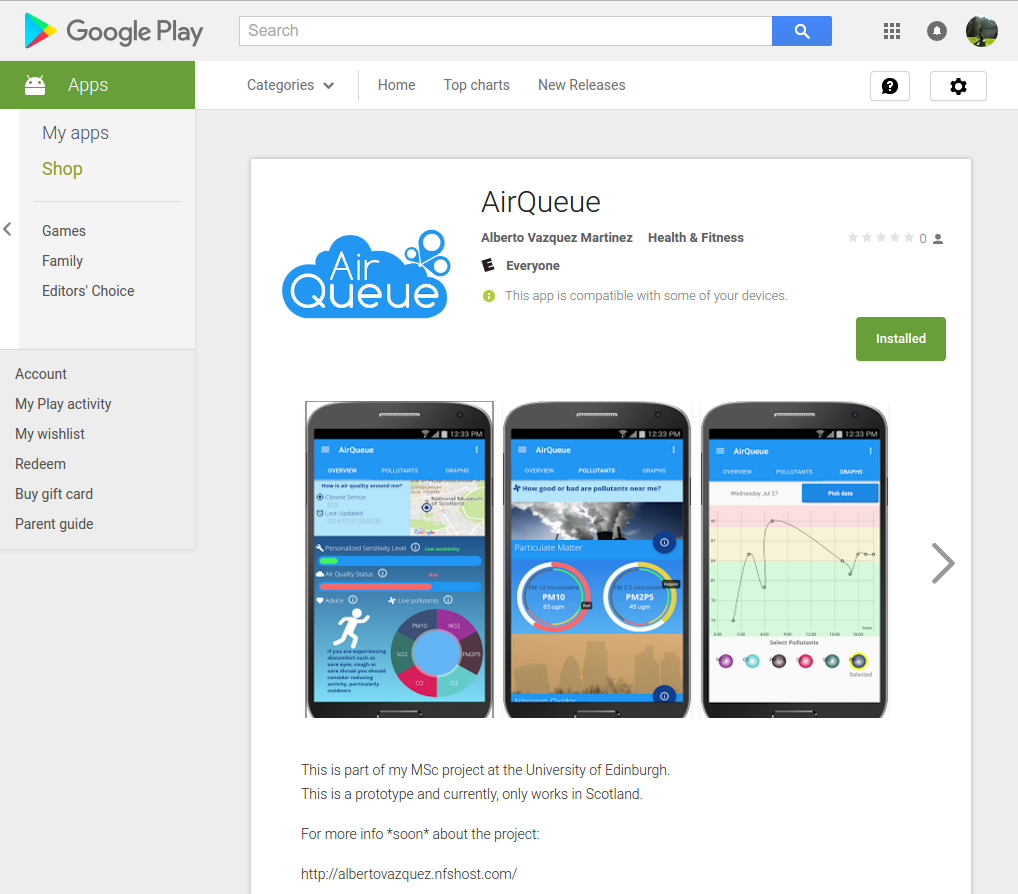
\includegraphics[scale=1]{images/play_store.png}
\end{adjustbox}
  \caption[Deployment on Google Play Store]{Deployment on Google Play Store.\footnotemark}
  \label{fig:deployment_play_store}
\end{figure}
\footnotetext{\url{https://play.google.com/store/apps/details?id=com.beto4812.airqueue&hl=en_GB}}


\chapter{Evaluation}
At this point, the development of the final product was extensively carried out with different design and development iterations with feedback received from the stakeholders. The web-crawler component of the back-end system has been already working for around two months; and many senor readings are available for the users to test with the real gathered data. However, because the air-quality levels in Scotland are always generally good; there was no space to showcase the full capabilities of the system, i.e, under very polluted environments. Because of this, a small 'demo mode' was added to the system to give the opportunity to experiment it under very polluted scenarios. 

\iffalse
\subsection{User sampling}
According to Scholtz \cite{Scholtz2003}, the evaluation should be realized with around 5 participants per representative class of users. Unfortunately, due to time restrictions, the evaluation was realized with only one class of users.The evaluation was carried out with 4 users, one of them individually, and other three users as a group. 
\fi

\section{Functional test}


Database performance: . The entire dataset weights less than 22 megabytes. The response time is extremely quick (in miliseconds). The scalability is automatic. 



Tested through the Amazon Mobile Hub



\section{Non functional test}

\subsection{Design critique}


The development of the system with the final requirements has been carried out. 
The testing method was as follows: An invitation was sent to the UK asthma advisory group inviting participants with at least a basic computational background (As the evaluation is targeting a mobile application, the feedback from non computer users would have been biased), and interest about tracking air quality. 
A video camera was recording the meeting room to gather the opinions and discussion about the system. 
Device logging. 
User logging. 
\chapter{Conclusions and Future Work}

\bibliography{mendeley}
\bibliographystyle{IEEEtranN}
\end{document}
